\documentclass[sigconf]{acmart}

\usepackage[english]{babel}
\usepackage{blindtext}
\usepackage{indentfirst}

% Copyright
\renewcommand\footnotetextcopyrightpermission[1]{} % removes footnote with conference info
\setcopyright{none}
%\setcopyright{acmcopyright}
%\setcopyright{acmlicensed}
%\setcopyright{rightsretained}
%\setcopyright{usgov}
%\setcopyright{usgovmixed}
%\setcopyright{cagov}
%\setcopyright{cagovmixed}

\settopmatter{printacmref=false, printccs=false, printfolios=true}

% DOI
\acmDOI{}

% ISBN
\acmISBN{}

%Conference
%\acmConference[Submitted for review to SIGCOMM]{}
%\acmYear{2018}
%\copyrightyear{}

%% {} with no args suppresses printing of the price
\acmPrice{}


\begin{document}
\title{Network-Ordered Paxos Reproduction: \\Milestone Report}

%\titlenote{Produces the permission block, and copyright information}
%\subtitle{Extended Abstract}

\author{Emma Dauterman, Zo{\"e} Bohn}
% \author{Firstname Lastname}
% \authornote{Note}
% \orcid{1234-5678-9012}
% \affiliation{%
%   \institution{Affiliation}
%   \streetaddress{Address}
%   \city{City} 
%   \state{State} 
%   \postcode{Zipcode}
% }
% \email{email@domain.com}

% The default list of authors is too long for headers}
\renewcommand{\shortauthors}{Dauterman, Bohn}

\begin{abstract}
We present our in-progress reproduction of the evaluation of Network-Ordered Paxos \cite{nopaxos} (NOPaxos) by Li et. al.. We describe the problem NOPaxos attempts to solve and discuss the throughput vs. latency and scaling results we are reproducing. Our reproduction is unique in that instead of using dedicated hardware, we are testing on a cloud platform, requiring us to implement ordered unreliable multicast in software.
\end{abstract}

\maketitle

\section{Introduction}

\indent Today's data center applications depend on replication to ensure data availability and transparently mask server failures. Unfortunately, consensus protocols like Paxos\cite{paxos,paxossimple} and Raft\cite{raft} that provide replication with strong consistency guarantees also impose a performance overhead. Network-Ordered Paxos\cite{nopaxos} (NOPaxos) dramatically reduces this performance overhead by splitting the replication responsibility between the network and protocol layers. The authors of NOPaxos present a new network primitive to do this: ordered unreliable multicast (OUM). 

OUM provides semantics strong enough to reduce overhead at the protocol layer, but weak enough that OUM can be implemented at near-zero-cost within a datacenter. OUM is asynchronous and unreliable, and it guarantees that all replicas receive messages in the same order. It also provides multicast drop detection: either every replica receives a message or a drop notification, or no replica receives a message or a drop notification, an all-or-nothing guarantee. All packets for a OUM group are routed through a single sequencer, which determines the global packet order. The authors describes three places in the network to implement the sequencer: 
\begin{enumerate}
\item In the switches themselves using P4 (although at the time of writing, programmable switches that could run this code were not commercially available)
\item In hardware middleboxes (what the authors use for most of their evaluation)
\item At end-hosts (no specialized hardware needed, provides throughput comparable to that of hardware middleboxes but with increased latency)
\end{enumerate}
OUM greatly simplifies the task of the protocol layer: instead of agreeing on the total ordering of client requests, now replicas only have to agree on which requests to execute and which to permanently ignore. 

We will attempt to reproduce the authors' findings that show that NOPaxos dramatically reduces the cost of replication, performs better than other consensus protocols, and scales with an increasing number of replicas. The authors show that NOPaxos achieves a throughput within 2\% and latency within 16 microseconds of an unreplicated system, better than any other consensus protocol (Figure 5 in NOPaxos paper\cite{nopaxos}). They also show that NOPaxos maintains a throughput comparable to an unreplicated system with an increasing number of replicas (Figure 8 in NOPaxos paper\cite{nopaxos}). We will attempt to reproduce these key results.

\section{Related Work}

Other consensus protocols have also tried to reduce the performance overhead of replication. Speculative Paxos\cite{specpaxos} and NetPaxos\cite{netpaxos} take a similar approach to NOPaxos by pushing functionality into the network. Speculative Paxos uses a Mostly-Ordered Multicast primitive that provides a best-effort ordering property, but because it is not a guarantee, both superquorums and speculation are necessary. NOPaxos avoids protocol complexity by pushing more responsibility into the network layer. On the other hand, NetPaxos moves Paxos logic into the switches (using P4), requiring switches to store the results of each consensus instance, which could become a large amount of state. While NetPaxos requires changes to the switch firmware, NOPaxos has much more realistic expectations of switches, requiring only the OUM primitive. 

FastPaxos\cite{fastpaxos}, Generalized Paxos\cite{generalizedpaxos}, and Egalitarian Paxos\cite{epaxos} (EPaxos) take a different approach by making no assumptions about the network. Fast Paxos allows clients to send operations directly to replicas to reduce overhead, but if multiple clients concurrently send operations, extra messages are required to determine ordering (NOPaxos relies on the network to do this). Generalized Paxos and EPaxos both exploit commutativity to improve performance: Generalized Paxos is a version of Fast Paxos that exploits commutativity, and EPaxos uses multiple leaders to propose and execute operations concurrently. For both Generalized Paxos and EPaxos, performance depends on the nature of the workload (i.e. the degree of commutativity), and so cannot achieve the consistency of performance across workloads in NOPaxos. However, these protocols make no assumptions about the network, and so are good choices outside datacenters.

The authors compare NOPaxos to a subset of these other protocols: Speculative Paxos, Fast Paxos, Paxos without modification, Paxos with adaptive batching, and an unreplicated system (no performance overhead). 

\section{Experiment Design}

Unlike the NOPaxos authors, we do not have a dedicated network of servers with which run our tests. Therefore, to evaluate NOPaxos, we used a network of Google Compute Engine (GCE) nodes on Google's gcloud platform. We initially planned to use Mininet, as this would allow us to implement the sequencer in the switches themselves, the most advantageous place with regards to performance according to the NOPaxos paper. However, we realized that Mininet might not allow us to measure microsecond-level latencies, and so we switched to the gcloud platform instead. Because we can't program switches or insert middleboxes in gcloud, we chose to use an end-host sequencer, essentially creating another GCE node to route all packets through. We must also adjust our setup given that gcloud does not support multicast. Per the suggestion of the NOPaxos authors, we are modifying the end-host sequencer to send individual copies of packets to each replica in place of multicast, although we recognize that this could potentially become a bottleneck.

To replicate Figure 5, we run with 5 replicas (as specified in \cite{nopaxos}) and 1 end-host sequencer. We couldn't perfectly reproduce the testbed network topology shown in Figure 3 in the NOPaxos paper\cite{nopaxos} as we are using GCE nodes and so can't build a fat-tree, but we use the same number of end-hosts. We run one dedicated client server and add more concurrent client threads to increase throughput as necessary for the reproduction. To replicate Figure 8 in the NOPaxos paper\cite{nopaxos}, we run with 3, 5, 7, and 9 replicas respectively. 

\begin{figure}[tp]
\centering
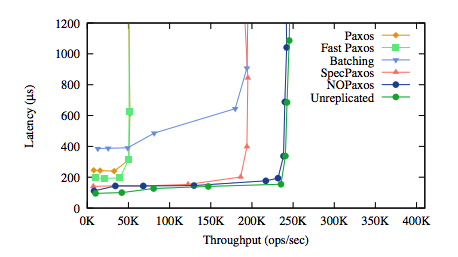
\includegraphics[scale=0.5]{figures/figure_5.png}
\caption{Original Figure 5 in \cite{nopaxos}, showing latency vs. throughput comparison for NOPaxos and other protocols}
\end{figure}

\begin{figure}[tp]
\centering
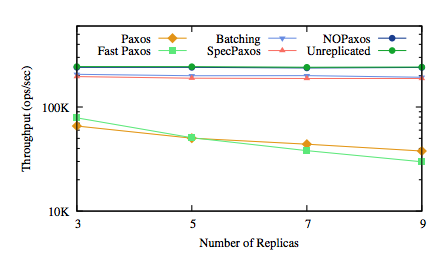
\includegraphics[scale=0.5]{figures/figure_8.png}
\caption{Original Figure 8 in \cite{nopaxos}, showing maximum throughput with increasing number of replicas}
\end{figure}


\section{Progress}

As described above, we initially planned to use Mininet and implement the sequencer in the switches, but after realizing that we couldn't measure microsecond-level latencies, we switched to a cloud platform and an end-host sequencer. According to the authors' measurements (Figure 6), the end-host sequencer achieves comparable throughput and increased latency (36\%) in comparison to the hardware middlebox implementation they test with. Thus our reproduction of Figure 5 will really be a combination of Figures 5 and 6: all of the protocols except NOPaxos in Figure 5 should be the same, but instead of NOPaxos, we'll measure NOPaxos + end-host sequencer (as shown in Figure 6 of the NOPaxos paper). Figure 8 should be unaffected as it only measures number of replicas and throughput, and the end-host sequencer and network processor have comparable throughput. 

\begin{figure}[tp]
\centering
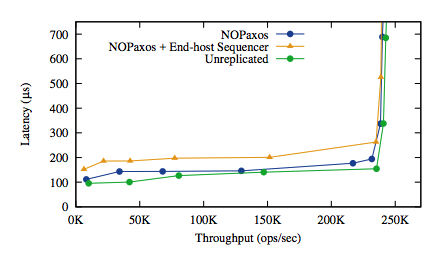
\includegraphics[scale=0.5]{figures/figure_6.png}
\caption{Original Figure 6 in \cite{nopaxos}, showing comparison of NOPaxos sequencers}
\end{figure}

The authors' implementation of the end-host sequencer leverages multicast, but most/all cloud platforms do not support multicast. When we reached out to the authors, they suggested that we modify the existing end-host sequencer to send a separate copy of the sequenced packet to each of the replicas. However, they think there's a chance the sequencer could become a bottleneck and affect the results, and so we will need to be aware of this as we gather data. 

The authors suggested these modifications to the end-host sequencer to send a separate copy of each packet to each replica:

\begin{enumerate}
  \item Add the endhost sequencer's address to configuration (lib/configuration.h, lib/configuration.cc)
  \item Ordered multicast messages should be sent to the sequencer's address, instead of the broadcast address (OrderedMulticast function in lib/udptransport.cc)
  \item The endhost sequencer currently ignores all non-broadcast messages. Remove those checks.
  \item Modify the sequencer to send individual packets to each replica. This is the most tricky part. The endhost sequencer does use raw socket. So you could directly modify the destination MAC address, IP address and the UDP port in the packet header.
\end{enumerate}

We have steps 1-3, and are currently in the process of debugging for step 4. 

We don't need the sequencer to run the other protocols, though, and we've set up our network and configuration files to take preliminary measurements for all other protocols measured in Figures 5 and 8: viewstamped replication\cite{vr} (which the authors use for regular paxos and paxos with batching), fast paxos, speculative paxos, and unreplicated.

The authors took their measurements with 5 replicas for Figure 5 and 3, 5, 7, and 9 replicas for Figure 8. We therefore set up 9 GCE nodes to act as replicas for us to take our measurements with. 

\begin{figure}[tp]
\centering
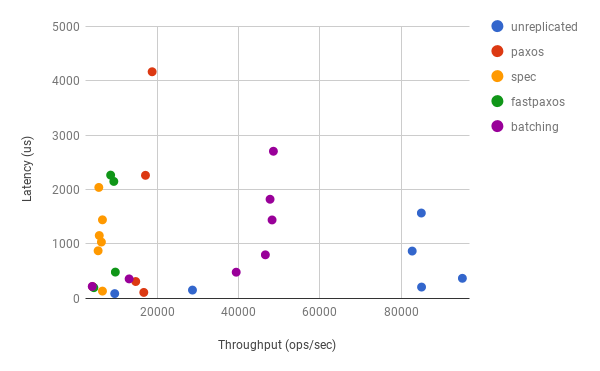
\includegraphics[scale=0.4]{figures/figure_5_2.png}
\caption{Our in-progress reproduction of figure 5 in \cite{nopaxos}, showing latency vs. throughput comparison for NOPaxos and other protocols}
\end{figure}

We began by taking measurements for the throughput and latency of a single client communicating with 5 replicas running each of paxos, paxos with batching, fast paxos, speculative paxos, and unreplicated. We used the benchmarking code in the authors' repository, which actually provides four different latency metrics (median and 90th, 95th, and 99th percentile). We again reached out to the authors to ask which of these metrics was used for Figure 5, and they indicated that they'd actually measured average latency (and very generously proceeded to push an update to the repository so that the benchmark code would output average latency as well). 

When looking at scaling the number of concurrent clients for Figure 5, we determined that although the existing benchmark code has an option for running multiple client threads, there is currently no code for combining the latency and throughput measurement of multiple clients on a given run. We therefore wrote a simple python script to combine these measurements ourselves.

We then proceeded to take throughput and latency measurements for multiple client threads. Our results are graphed in Figure 4 of this paper, our in-progress reproduction of Figure 5 in \cite{nopaxos}. As is clear from the figure, the levels of throughput we were able to achieve by scaling the number of threads was still significantly lower than what the authors were able to achieve. This is likely a result of the fact that we are running these protocols over the distributed, multi-user google cloud platform, whereas the authors were able to use dedicated hardware all in the same location. However, the general distribution of performance is still similar; in particular, it is still clear that the paxos with batching and unreplicated protocols perform better than the fastpaxos and vanilla paxos protocols. Speculative paxos is currently an outlier for us as replicas began crashing when we ran with more than 5-10 threads. 

We next took a preliminary set of throughput measurements for Figure 8 for paxos, fast paxos, speculative paxos, and unreplicated when running with 3, 5, 7, and 9 servers with a single client. We immediately saw that our numbers were an order of magnitude lower than the authors’ for Figure 8. We therefore concluded that the authors were measuring the throughput for a larger number of concurrent clients, as in Figure 5, and will therefore repeat these measurements once our reproduction of Figure 5 is complete. 

\section{Next Steps}
In our remaining time, we plan to accomplish the following tasks:

\begin{enumerate}
  \item Finish implementing and debugging the end-host sequencer. This should allow us to begin collecting measurements for NOPaxos.
  \item Investigate why specpaxos fails with 5-10 client threads.
  \item Finish collecting data for Figure 5.
  \item Repeat data collection for Figure 8 with a larger number of concurrent clients.
  \item Compare with the authors' results to see if our implementation of the sequencer without multicast becomes a bottleneck.
\end{enumerate}

If we have more time, we plan on investigating the effects of multiple OUM groups, each with their own end-host sequencer, to test if the sequencer is a bottleneck, and, if so, how the number of sequencers affects throughput and latency.




\bibliographystyle{ACM-Reference-Format}
\bibliography{reference}

\end{document}